%!TEX root = ../bachelorthesis.tex
\chapter{Architektur}
Für dieses Projekt wurden mehrere Softwareprogramme integriert. In den folgenden Kapiteln wird ein Gesamtüberblick gegeben und die einzelnen Teile werden detailliert beschrieben.

\section{Gesamtübersicht} % (fold)
\label{sec:gesamtübersicht}
In \autoref{img:overview} ist die Architektur graphisch dargestellt. Jedes Element stellt dabei eine ROS-Node dar, also ein einzelnes Programm.

\begin{figure}[!hbt]
	\centering
	\vspace{1ex}
	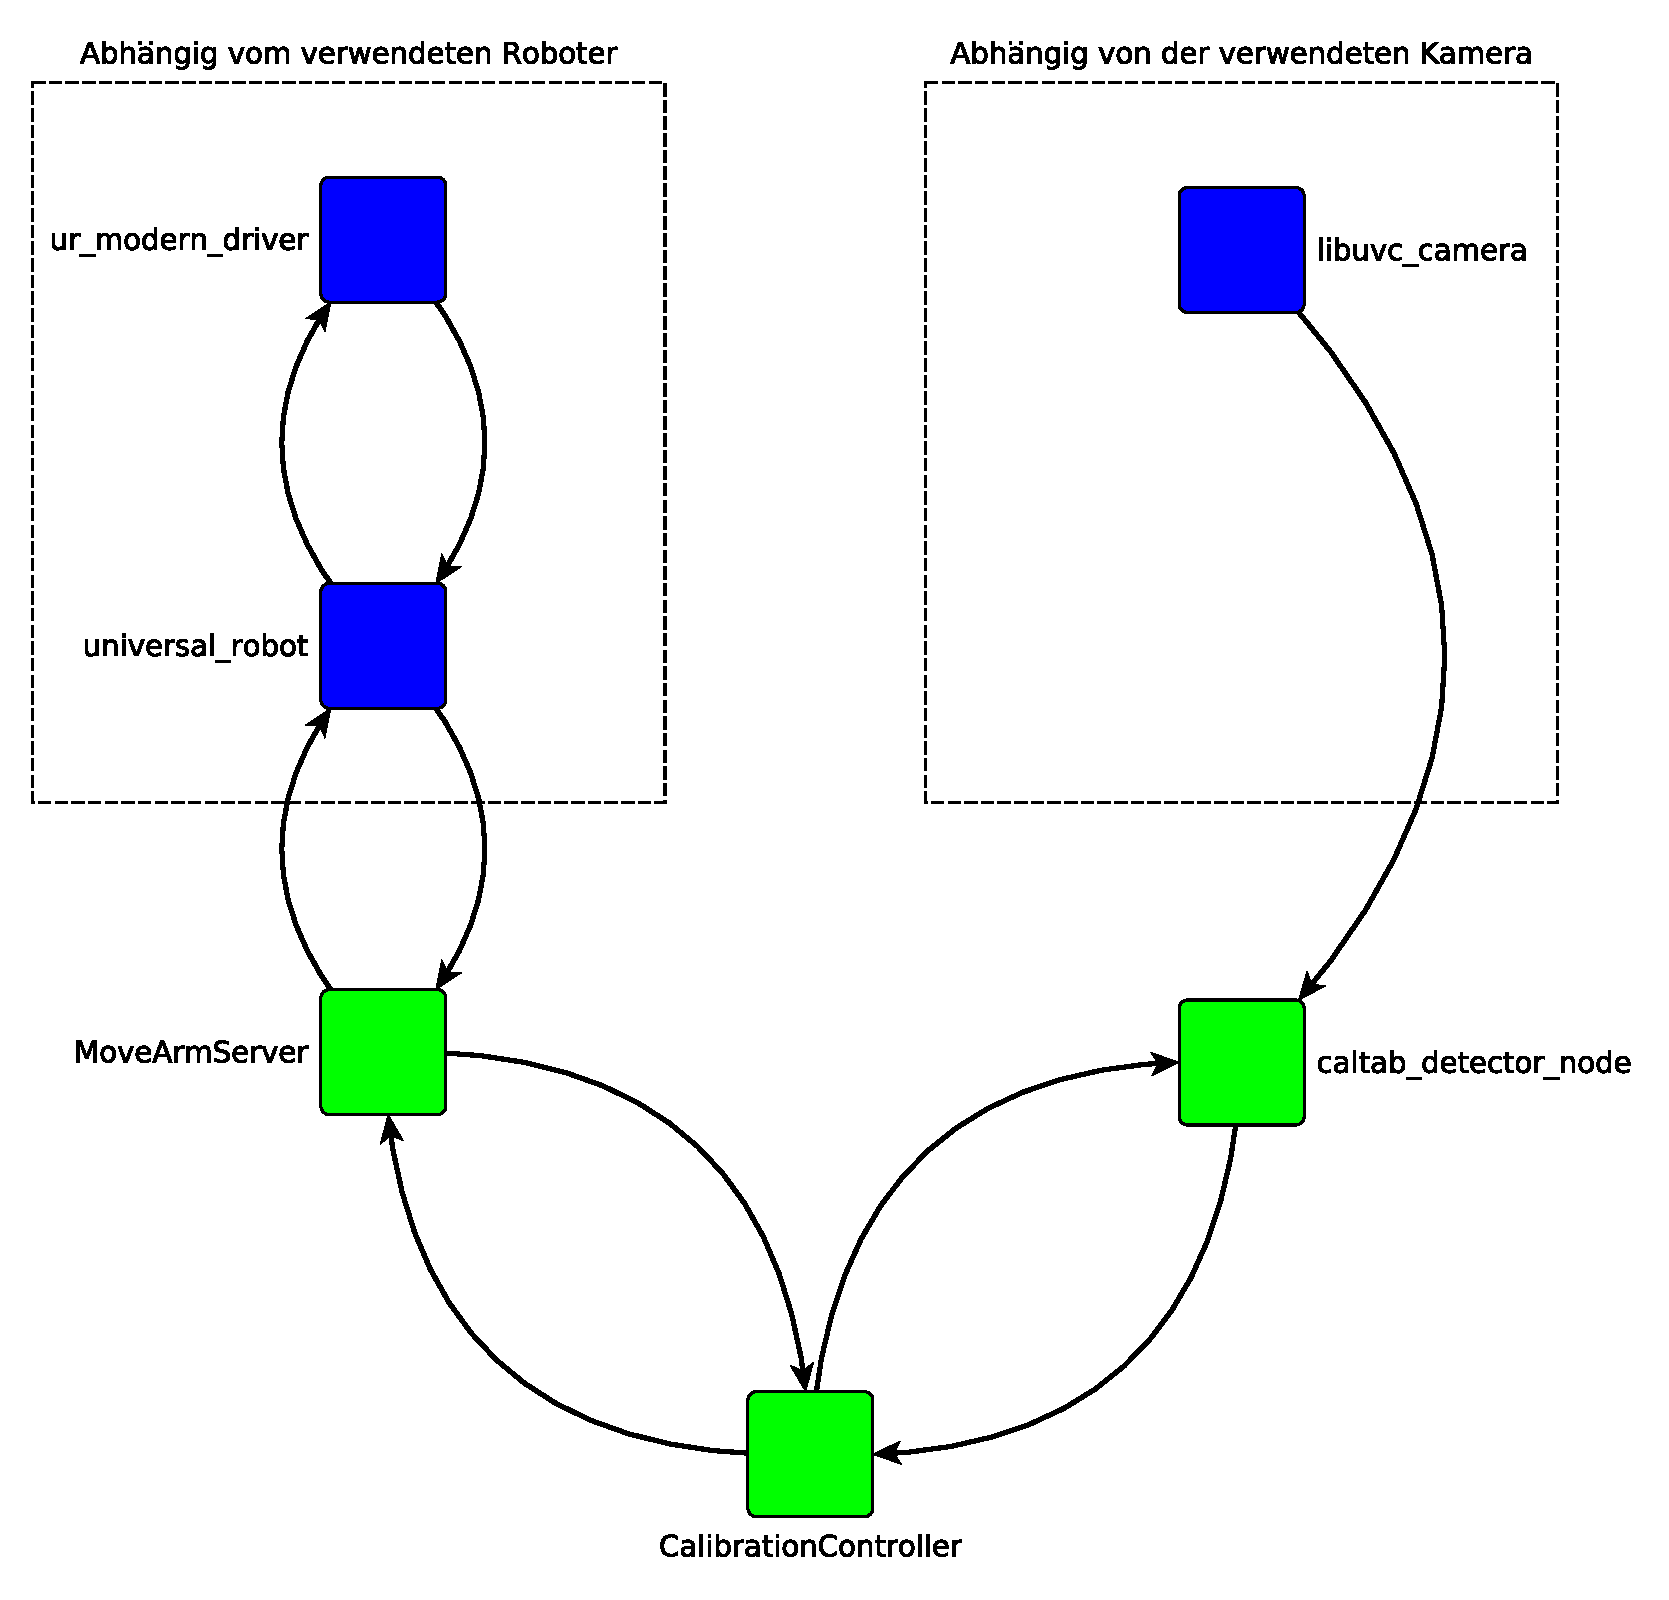
\includegraphics[scale=0.6]{../images/overview}
	\caption[Übersicht über die Architektur]{\label{img:overview} Übersicht über die Architektur}
	\vspace{1ex}
\end{figure}

Die beiden dunkelblauen Elemente ur\_moder\_driver und libuvc\_camera steuern direkt die Hardware an. im Fall von ur\_modern\_driver wird der UR5-Arm gesteuert, libuvc\_camera steuert die Webcam.

Das hellblaue Element universal\_robot stellt eine abstrahierte Schnittstelle zur Steuerung des Roboterarms zur Verfügung.

Die beiden grünen Elemente MoveArmServer und caltab\_detector\_node wurden im Rahmen dieser Bachelorarbeit geschrieben. MoveArmServer bietet Funktionen zur Steuerung des Arms, die speziell in diesem Projekt benötigt werden. caltab\_detector\_node kümmert sich um das Verarbeiten der Bildinformationen.

Das gelbe Element CalibrationController wurde ebenfalls im Rahmen dieser Bachelorarbeit entwickelt. Dieses Programm steuert den gesamten Ablauf, kommuniziert mit den beiden gelben Elementen und sorgt dafür, dass der Roboter sich an die gewünschten Positionen bewegt und die Bilder im richtigen Moment aufgenommen werden. Zum Schluss werden dem Benutzer dann die ermittelten Parameter zurückgegeben.

\section{ur\_modern\_driver} % (fold)
\label{sec:ur_modern_driver}
Diese Node wurde bereits als Paket in ROS veröffentlicht, siehe \cite{ur_modern_driver}. Sie bietet eine Schnittstelle zwischen dem Roboterarm UR5 und dem ROS Framework. Da dieses Paket nicht für die in diesem Projekt benutzte ROS Version entwickelt wurde, mussten einige wenige Anpassungen am Sourcecode vorgenommen werden, um das Paket in diesem Projekt zu benutzen.

\section{universal\_robot} % (fold)
\label{sec:universal_robot}
Diese Node wurde ebenfalls als Paket in ROS veröffentlicht, siehe \cite{universal_robot}. In dieser Node ist MoveIt! integriert, welches zum Bewegen des Roboterarms benutzt wird. Man kann diesem Programm die gewünschte Position und Orientierung des Roboterarms übergeben, und das Programm führt die erforderliche Bewegung dann durch, sofern die Position und Orientierung für den Arm erreichbar sind.

An diesem Programm wurden einige Anpassungen vorgenommen. Zum einen wurde die in MoveIt! benutzte Bibliothek zur Lösung der inversen Kinematik KDL durch TRAC\_IK ausgetauscht. Während der Versuche kam es vor, dass MoveIt! keinen oder nur einen viel zu komplizierten Weg von der Start zur Zielkonfiguration gefunden hat. Dieses Problem konnte teilweise durch diesen Austausch behoben werden.

Zusätzlich wurde das URDF in diesem Paket angepasst. Das URDF enthält geometrische Informationen über den Roboterarm wie z.B. die Länge und Form der einzelnen Glieder. Im Standardfall soll der Endpunkt des Roboterarms an die übergeben Position bewegt werden. In diesem Projekt ist allerdings das Kalibrierungsmuster an dem Endpunkt befestigt. Es ist allerdings nicht mittig an dem Punkt montiert sondern steht zu einer Seite ab. Daher wurde das URDF so verändert, dass nun der Mittelpunkt des Musters der Endpunkt für den Roboterarm ist. Dadurch lässt sich das Muster einfacher an die gewünschten Positionen bewegen.

Diese Node wird im Projekt von dem Programm MoveArmServer angesprochen. Dazu stellt sie über MoveIt! einige Schnittstellen bereit, die in diesem Fall benutzt werden, um die Position und Orientierung des Kalibrierungsmusters zu verändern.

\section{libuvc\_camera} % (fold)
\label{sec:libuvc_camera}
Auch diese Node ist als Paket in ROS verfügbar. Sie dient dazu, das Bild der angeschlossen Webcam über ROS verfügbar zu machen. In dem Script, mit dem diese Node gestartet wird, lassen sich verschiedene Parameter einstellen. In diesem Fall wurde mittels der Vendor-ID und Product-ID die zu benutzende Kamera definiert, die Auflösung wurde auf Full-HD gesetzt und der Fokus wird so eingestellt, dass der Bereich, in dem sich das Kalibrierungsmuster befinden wird, scharf zu sehen ist.

Die Node veröffentlicht die Bilder der Kamera über sogenannte Topics. Das Programm caltab\_detector\_node empfängt die Bilder und wertet sie aus.

\section{MoveArmServer} % (fold)
\label{sec:movearmserver}
Dieses Programm wurde im Rahmen dieser Bachelorarbeit selber entwickelt. Es dient dazu, dem CalibrationController eine weitere Abstraktionsschicht zum Bewegen des Arms zu bieten.

Dazu wurde ein Actionserver erstellt, der die Position des Kalibrierungsmusters als Auftrag erhält. Zusätzlich kann als weiterer Parameter für den Auftrag die Neigung des Musters angegeben werden. Das Programm berechnet dann für die gewünschte Position zunächst die Orientierung für das Muster damit dieses senkrecht zur Kamera steht. Anschließend wird die Orientierung mit der gewünschten Neigung berechnet. Diese Zielkonfiguration wird dann an MoveIt! übergeben. Abhängig davon, ob MoveIt! den Arm erfolgreich bewegen konnte oder nicht, informiert der MoveArmServer den CalibrationController, ob der Auftrag erfolgreich ausgeführt wurde oder nicht.

\section{caltab\_detector\_node} % (fold)
\label{sec:caltab_detector_node}
Auch dieses Programm wurde selbst entwickelt. Es benutzt die Bibliothek von HALCON, um in den Bildern, die es von der Kamera empfängt, nach dem Kalibrierungsmuster zu suchen und die Kalibrierung durchzuführen.

Diese Node bietet zwei Actionserver an. Der erste Actionserver erwartet einen Auftrag, um in den aktuellen Bildern nach dem Kalibrierungsmuster zu suchen. Dazu wird ein Parameter übergeben, wie viele Bilder ausgewertet werden sollen. Die Algorithmen von HALCON finden nicht immer im ersten Versuch das Muster, daher lässt sich die Anzahl der Bilder definieren. Die Node meldet dem CalibrationController zurück, ob nach der angegeben Anzahl der Bilder das Muster gefunden wurde oder nicht.

Der zweite Actionserver nimmt den Auftrag zur Durchführung der Kalibrierung an. Dazu werden die Bilder, in denen das Muster zu sehen war, ausgewertet. Danach werden die errechneten intrinsischen Parameter, die Verzeichnungsparameter sowie der ermittelte durchschnittliche Fehler an den CalibrationController zurückgegeben.

\section{CalibrationController} % (fold)
\label{sec:calibrationcontroller}
Diese letzte Node wurde ebenfalls selbst entwickelt. Sie dient dazu, den gesamten Ablauf der Kalibrierung zu steuern, indem sie die Actionserver mit Aufgaben versorgt. Zunächst übergibt der Benutzer dem Programm die Position der Kamera in Relation zur Basis des Roboterarms und die initialen intrinsischen Parameter. Dann wird aus diesen Werten das Sichtfeld der Kamera bestimmt. Mit diesem Sichtfeld werden dann die verschiedenen Distanzen zur Kamera berechnet und anschließend die Positionen für das Kalibrierungsmuster, damit dieses das ganze Sichtfeld der Kamera abdeckt.

Diese Positionen werden der Reihe nach an den MoveArmServer übergeben. Für jede Position wird das Muster für um 10$^\circ$, 20$^\circ$, 30$^\circ$ und 40$^\circ$ nach oben, unten, rechts und links geneigt. Hat der Actionserver den Auftrag erfolgreich ausgeführt, wird der caltab\_detector\_node der Auftrag übergeben, in dem Kamerabild nach dem Muster zu suchen. Ist dieser Auftrag abgeschlossen, wird die nächste Position angesteuert.

Wurden alle Positionen abgearbeitet, wird zum Schluss der Auftrag zur Kalibrierung durchgeführt. Die dadurch erhaltenen Parameter werden dem Benutzer angezeigt und das Programm hat seine Durchführung beendet.